\documentclass{article}
\usepackage{physics}
\usepackage{graphicx}
\usepackage{caption}
\usepackage{amsmath}
\usepackage{bm}
\usepackage{framed}
\usepackage{authblk}
\usepackage{empheq}
\usepackage{amsfonts}
\usepackage{esint}
\usepackage[makeroom]{cancel}
\usepackage{dsfont}
\usepackage{centernot}
\usepackage{mathtools}
\usepackage{subcaption}
\usepackage{bigints}
\usepackage{amsthm}
\theoremstyle{definition}
\newtheorem{lemma}{Lemma}
\newtheorem{defn}{Definition}[section]
\newtheorem{prop}{Proposition}[section]
\newtheorem{rmk}{Remark}[section]
\newtheorem{thm}{Theorem}[section]
\newtheorem{exmp}{Example}[section]
\newtheorem{prob}{Problem}[section]
\newtheorem{sln}{Solution}[section]
\newtheorem*{prob*}{Problem}
\newtheorem{exer}{Exercise}[section]
\newtheorem*{exer*}{Exercise}
\newtheorem*{sln*}{Solution}
\usepackage{empheq}
\usepackage{tensor}
\usepackage{xcolor}
%\definecolor{colby}{rgb}{0.0, 0.0, 0.5}
\definecolor{MIT}{RGB}{163, 31, 52}
\usepackage[pdftex]{hyperref}
%\hypersetup{colorlinks,urlcolor=colby}
\hypersetup{colorlinks,linkcolor={MIT},citecolor={MIT},urlcolor={MIT}}  
\usepackage[left=1in,right=1in,top=1in,bottom=1in]{geometry}
\usepackage[figurename=Fig.]{caption}

\usepackage{newpxtext,newpxmath}
\newcommand*\widefbox[1]{\fbox{\hspace{2em}#1\hspace{2em}}}

\newcommand{\p}{\partial}
\newcommand{\R}{\mathbb{R}}
\newcommand{\C}{\mathbb{C}}
\newcommand{\lag}{\mathcal{L}}
\newcommand{\nn}{\nonumber}
\newcommand{\ham}{\mathcal{H}}
\newcommand{\M}{\mathcal{M}}
\newcommand{\I}{\mathcal{I}}
\newcommand{\K}{\mathcal{K}}
\newcommand{\F}{\mathcal{F}}
\newcommand{\w}{\omega}
\newcommand{\lam}{\lambda}
\newcommand{\al}{\alpha}
\newcommand{\be}{\beta}
\newcommand{\x}{\xi}

\newcommand{\G}{\mathcal{G}}

\newcommand{\f}[2]{\frac{#1}{#2}}

\newcommand{\ift}{\infty}

\newcommand{\lp}{\left(}
\newcommand{\rp}{\right)}

\newcommand{\lb}{\left[}
\newcommand{\rb}{\right]}

\newcommand{\lc}{\left\{}
\newcommand{\rc}{\right\}}


\newcommand{\V}{\mathbf{V}}
\newcommand{\U}{\mathcal{U}}
\newcommand{\Id}{\mathcal{I}}
\newcommand{\D}{\mathcal{D}}
\newcommand{\Z}{\mathcal{Z}}

%\setcounter{chapter}{-1}


\usepackage{enumitem}



\usepackage{listings}
\captionsetup[lstlisting]{margin=0cm,format=hang,font=small,format=plain,labelfont={bf,up},textfont={it}}
\renewcommand*{\lstlistingname}{Code \textcolor{violet}{\textsl{Mathematica}}}
\definecolor{gris245}{RGB}{245,245,245}
\definecolor{olive}{RGB}{50,140,50}
\definecolor{brun}{RGB}{175,100,80}

%\hypersetup{colorlinks,urlcolor=colby}
\lstset{
	tabsize=4,
	frame=single,
	language=mathematica,
	basicstyle=\scriptsize\ttfamily,
	keywordstyle=\color{black},
	backgroundcolor=\color{gris245},
	commentstyle=\color{gray},
	showstringspaces=false,
	emph={
		r1,
		r2,
		epsilon,epsilon_,
		Newton,Newton_
	},emphstyle={\color{olive}},
	emph={[2]
		L,
		CouleurCourbe,
		PotentielEffectif,
		IdCourbe,
		Courbe
	},emphstyle={[2]\color{blue}},
	emph={[3]r,r_,n,n_},emphstyle={[3]\color{magenta}}
}






\begin{document}
\begin{framed}
\noindent Name: \textbf{Huan Q. Bui}\\
Course: \textbf{8.422 - AMO II}\\
Problem set: \textbf{\#2}\\
Due: Friday, Feb 24, 2022\\
References: Help from TA Eric Wolf
\end{framed}
	
	




\noindent \textbf{1. When the mechanical momentum is not the canonical momentum}

\noindent In this problem we will see that the motion of neutral atoms in a rotating frame can be described as the motion of a charged particle experiencing a scalar potential and an effective magnetic field. Consider free motion in the $xy$-plane. The transformation from the lab from to a frame rotating at angular frequency $\Omega$ about the $z$-axis is 
\begin{align*}
	\begin{pmatrix}
		\tilde{x}(t) \\  \tilde{y}(t)
	\end{pmatrix}
	= 
	\begin{pmatrix}
		\cos \Omega t  & \sin\Omega t \\ -\sin\Omega t & \cos\Omega t 
	\end{pmatrix}
	\begin{pmatrix}
		x(t) \\ y(t)
	\end{pmatrix}
	&\implies 
	\begin{pmatrix}
		{x}(t) \\  {y}(t)
	\end{pmatrix}
	= 
	\begin{pmatrix}
		\cos \Omega t  & -\sin\Omega t \\ \sin\Omega t & \cos\Omega t 
	\end{pmatrix}
	\begin{pmatrix}
		\tilde{x}(t) \\ \tilde{y}(t)
	\end{pmatrix} \\
	& \implies
	\begin{pmatrix}
		\dot{x}(t) \\  \dot{y}(t)
	\end{pmatrix}
	= 
	\begin{pmatrix}
		-\Omega \sin \Omega t  & -\Omega \cos\Omega t \\ \Omega \cos\Omega t & \Omega \sin\Omega t 
	\end{pmatrix} \begin{pmatrix}
	\tilde{x}(t) \\ \tilde{y}(t)
\end{pmatrix}
	+ 
	\begin{pmatrix}
	\cos \Omega t  & -\sin\Omega t \\ \sin\Omega t & \cos\Omega t 
	\end{pmatrix}
	\begin{pmatrix}
	\dot{\tilde{x}}(t) \\ \dot{\tilde{y}}(t)
	\end{pmatrix}
\end{align*}



\begin{enumerate}[label=\alph*)]
	\item The kinetic energy of a particle of mass $m$ in terms of the coordinates and velocities in the rotating frame is 
	\begin{align*}
		T 
		&= \f{1}{2} m (\dot{x}^2 + \dot{y}^2)\\ 
		&= \f{1}{2}m \lb \Omega^2 (\tilde{x}^2 + \tilde{y}^2) + 2\Omega (\tilde{x}\dot{\tilde{y}} - \dot{\tilde{x}}\tilde{y}) + (\dot{\tilde{x}}^2 + \dot{\tilde{y}}^2)  \rb \\
		&= {\f{1}{2}m \lb  ( \dot{\tilde{x}} - \Omega \tilde{y})^2 + (\dot{\tilde{y}} + \Omega \tilde{x} )^2 \rb}.
	\end{align*}
	
	\item The Lagrangian is just the kinetic energy from above:
	\begin{align*}
		\lag(\tilde{x}, \tilde{y}, \dot{\tilde{x}}, \dot{\tilde{y}}, t) =  {\f{1}{2}m \lb  ( \dot{\tilde{x}} - \Omega \tilde{y})^2 + (\dot{\tilde{y}} + \Omega \tilde{x} )^2 \rb}.
	\end{align*}
	The canonical momenta are therefore
	\begin{align*}
		\tilde{p}_x &= \f{\p \lag}{\p \dot{\tilde{x}}} = m(\dot{\tilde{x}} - \Omega \tilde{y}) \\
		\tilde{p}_y &= \f{\p \lag}{\p \dot{\tilde{y}}} = m(\dot{\tilde{y}} + \Omega \tilde{x}).
	\end{align*}
	
	\item By inspection, $\{\tilde{x}, \tilde{p}_x\} = 1$ and $\{ \tilde{p}_i, \tilde{p}_j \} = \delta_{ij}$. Now we look at  
	\begin{align*}
		\{ m\dot{\tilde{x}}, m\dot{\tilde{y}} \} &= m^2\lp \f{\p \dot{\tilde{x}} }{\p \tilde{x}}
		{\f{\p \dot{\tilde{y}} }{\p \tilde{p}_x}} - \f{\p \dot{\tilde{y}}}{\p \tilde{x}}\f{\p \dot{\tilde{x}}}{\p \tilde{p}_x}\rp + 
		m^2\lp \f{\p \dot{\tilde{x}} }{\p \tilde{y}}\f{\p \dot{\tilde{y}} }{\p \tilde{p}_y} - \f{\p \dot{\tilde{y}}}{\p \tilde{y}} {\f{\p \dot{\tilde{x}}}{\p \tilde{p}_y}}\rp.
	\end{align*}
	From $m\dot{\tilde{x}} = \tilde{p}_x + m\Omega \tilde{y}$ and $m\dot{\tilde{y}} = \tilde{p}_y - m\Omega \tilde{x}$ we find 
	\begin{align*}
		\{ m\dot{\tilde{x}}, m\dot{\tilde{y}} \} 
		&= m^2\lp \cancel{\f{\p \dot{\tilde{x}} }{\p \tilde{x}}}
		\cancel{\f{\p \dot{\tilde{y}} }{\p \tilde{p}_x}} - \f{\p \dot{\tilde{y}}}{\p \tilde{x}}\f{\p \dot{\tilde{x}}}{\p \tilde{p}_x}\rp + 
		m^2\lp \f{\p \dot{\tilde{x}} }{\p \tilde{y}}\f{\p \dot{\tilde{y}} }{\p \tilde{p}_y} -\cancel{ \f{\p \dot{\tilde{y}}}{\p \tilde{y}}} \cancel{\f{\p \dot{\tilde{x}}}{\p \tilde{p}_y}}\rp\\
		&= m^2\lp-\f{-\Omega}{m}\rp + m^2\lp \f{\Omega}{m} \rp \\
		&= {2m\Omega \neq 0 \text{ if } \Omega \neq 0}
	\end{align*}
	
	\item The Hamiltonian is the Legendre transform of the Lagrangian:
	\begin{align*}
		\ham 
		= \lp \dot{\tilde{x}}\tilde{p}_x + \dot{\tilde{y}}\tilde{p}_y \rp - \lag 
		= \f{\tilde{p}_x^2}{2m} +\f{\tilde{p}_y^2}{2m} - \Omega (\tilde{x}  \tilde{p}_y  -  \tilde{y} \tilde{p}_x)
	\end{align*}
	where we have written $\dot{\tilde{x}}$ and $\dot{\tilde{y}}$ in terms of $\tilde{p}_x,\tilde{p}_y,\tilde{x},\tilde{y}$. We shall complete the squares to get
	\begin{align*}
		\ham 
		&= \f{\tilde{p}_x^2 + 2 m\Omega \tilde{p}_x\tilde{y} + m^2\Omega^2 \tilde{y}^2}{2m} + 
		\f{\tilde{p}_y^2 - 2 m\Omega \tilde{p}_y\tilde{x} + m^2\Omega^2 \tilde{x}^2}{2m} - \f{1}{2}m\Omega^2 (\tilde{x}^2 + \tilde{y}^2) \\ 
		&= \f{(\tilde{p}_x + m\Omega \tilde{y})^2 + (\tilde{p}_y - m\Omega \tilde{x})^2}{2m} - \f{1}{2}m\Omega^2 (\tilde{x}^2 + \tilde{y}^2) \\
		&= \f{(\vec{\tilde{p}} - q\vec{A})^2}{2m}  - \f{1}{2}m\Omega^2 (\tilde{x}^2 + \tilde{y}^2)\\
		&= \f{(\vec{\tilde{p}} - q\vec{A})^2}{2m} + V_\text{eff}(\tilde{x}, \tilde{y}).
	\end{align*}
	Here, we have re-written the Hamiltonian in terms of the vector potential $\vec{A}$ where $q\vec{A} = m \vec{\Omega} \times \vec{\tilde{r}} = (-m\Omega \tilde{y}, m\Omega \tilde{x},0)$ and an effective scalar potential $V_\text{eff}(\tilde{x}, \tilde{y}) = -m\Omega^2 (\tilde{x}^2 + \tilde{y}^2)/2$, which we may refer to as the centrifugal potential. In terms of electromagnetic theory, this "mechanical" potential can be rewritten as $V_\text{eff}= q \phi$ where $\phi(\tilde{x},\tilde{y}) =  -m\Omega^2 (\tilde{x}^2 + \tilde{y}^2)/2q$ is the electric (scalar) potential. The effective magnetic field $\vec{B}$ associated with the vector potential $\vec{A}$ is 
	\begin{align*}
		\vec{B} = \grad \times \vec{A} = \f{2m\Omega}{q} \hat{z} = \f{2m\Omega}{q} \hat{\tilde{z}}.
	\end{align*}
	The electric field associated with $\phi$ and $\vec{A}$ is 
	\begin{align*}
		\vec{E} =  - \grad \phi - \f{\p \vec{A}}{\p t} = \f{m\Omega^2}{q}\begin{pmatrix}
			\tilde{x} \\ \tilde{y} \\ 0
		\end{pmatrix}
	- \begin{pmatrix}
		\p_t A_x \\ \p_t A_y \\ 0
	\end{pmatrix}.
	\end{align*}


	\item The Hamiltonian not in terms of $\vec{A}$ and $V_\text{eff}$ is 
	\begin{align*}
		\ham = \f{\tilde{p}_x^2}{2m} +\f{\tilde{p}_y^2}{2m} - \Omega (\tilde{x}  \tilde{p}_y  -  \tilde{y} \tilde{p}_x)
	\end{align*}
	Compared to the original Hamiltonian, $\ham_\text{inertial} = p_x^2/2m + p_y^2/2m$, we see that there is an additional operator 
	\begin{align*}
		W(\tilde{x},\tilde{y}, \tilde{p}_x, \tilde{p}_y) = - \Omega (\tilde{x}  \tilde{p}_y  -  \tilde{y} \tilde{p}_x)
	\end{align*}
	This operator suffices for describing motion of the particle in the rotating frame because $L_z = \tilde{x}  \tilde{p}_y  -  \tilde{y} \tilde{p}_x$ is the generator of rotation about the $z$-axis. To see a deep reason for \textit{why} this term is all is needed, we have to look at infinitesimal canonical transformations and generating functions.  See these \href{https://ocw.mit.edu/courses/8-09-classical-mechanics-iii-fall-2014/f00f7f68ac7ba346a0868efb7430582c_MIT8_09F14_Chapter_4.pdf}{\underline{lecture notes}} for details. 
	
	\item The equations of motion for the particle in the rotating frame are gotten from Hamilton's equations of motion:
	\begin{align*}
		m\dot{\tilde{x}} &= m\f{\p \ham}{\p \tilde{p}_x} = \tilde{p}_x - q A_x \\ 
		m\dot{\tilde{y}} &= m\f{\p \ham}{\p \tilde{p}_y} = \tilde{p}_y - q  A_y \\
		\dot{\tilde{p}}_x &= -\f{\p \ham}{\p \tilde{x}} = \Omega \tilde{p}_y \\
		\dot{\tilde{p}}_y &= -\f{\p \ham}{\p \tilde{y}} = -\Omega \tilde{p}_x.
	\end{align*}
	From these we find 
	\begin{align*}
	m\ddot{\tilde{r}} 
	&= 	m\f{d^2}{dt^2} \begin{pmatrix}
			\tilde{x} \\ \tilde{y}
		\end{pmatrix}\\
	&= \begin{pmatrix}
		\Omega \tilde{p}_y - q\p_t A_x\\
		-\Omega \tilde{p}_x - q\p_t A_y
	\end{pmatrix}\\
	&= \begin{pmatrix}
		m\Omega (\dot{\tilde{y}} + \Omega \tilde{x}) - q \p_t A_x \\ 
		-m\Omega(\dot{\tilde{x}} - \Omega \tilde{y}) -q \p_t A_y
	\end{pmatrix} \\
	&= \begin{pmatrix}
		m\Omega \dot{\tilde{y}} \\ -m\Omega \dot{\tilde{x}}
	\end{pmatrix}
	+ \begin{pmatrix}
		m\Omega^2 \tilde{x} - q\p_t A_x \\ m\Omega^2 \tilde{y} - q \p_t A_y
	\end{pmatrix}\\
	&= q \tilde{\vec{v}} \times \vec{B} + q \vec{E}.
	\end{align*}
	Here we have ignored writing the $z$-components in the vector quantities for short. The expressions for $\vec{B}$ and $\vec{E}$ in terms of the quantities that appear in these equations come from Part (d). \\
	
	
	\noindent In the rotating frame, the particle behaves like a charged particle experiencing a Lorentz force (combination of the electric force and magnetic force) due to an effective electric and magnetic field. 
	
	
\end{enumerate}



\noindent \textbf{2. Quantum description of a charged particle in a uniform magnetic field - Landau levels.}

\noindent The Hamiltonian for a charged particle of charge $q>0$ moving freely in the $x-y$ plane in a uniform magnetic field $\vec{B} = B\hat{z}$ pointing along the $z$-axis is
\begin{align*}
	\ham = \f{1}{2m}\lp \vec{p} - q\vec{A} \rp^2.
\end{align*}
Let us ignore motion along $z$ and use the symmetric gauge $\vec{A} = -\vec{r}\times \vec{B}/2 = (-yB/2, xB/2,0)$. 

\begin{enumerate}[label=\alph*)]
	
	\item We obtain the classical equations of motion using the Lorentz force:
	\begin{align*}
		m\ddot{r} = q\vec{E} + q \vec{v}\times \vec{B} = q \vec{v} \times \vec{B}
	\end{align*}
	since we have implicitly assumed $\phi = 0$ by writing the Hamiltonian that way. In component form, this equation is 
	\begin{align*}
		\begin{pmatrix}
			\ddot{x} \\ \ddot{y}
		\end{pmatrix}
	= \f{qB}{m}\begin{pmatrix}
		\dot{y} \\ -\dot{x}  
	\end{pmatrix} 
	\end{align*}
	From here we get two second-order equations for $v_x$ and $v_y$: 
	\begin{align*}
		\ddot{v}_x = -\omega_c^2 v_x \quad\quad \ddot{v}_y = -\omega_c^2 v_y.
	\end{align*}
	where $\omega_c = qB/m$ is the cyclotron frequency. From the setup, we see that $v_x$ and $v_y$ are 90 degrees out of phase, so the motion is circular. The classical equations of motion are therefore
	\begin{align*}
		\ddot{x} = -\omega_c x \quad\quad \ddot{y} = -\omega_c^2 y 
	\end{align*}
	where $x^2 + y^2 = r_0^2 $ is constant. Assuming that the center of the orbit is $x_0$ and $y_0$, the classical trajectory of the particle is given by 
	\begin{align*}
		x(t) = x_0 + r_0\cos(\omega_c t ) \quad\quad 
		y(t) = y_0 - r_0\sin(\omega_c t ),
	\end{align*}
	since the particle moves clockwise for $q>0$ and $B$ pointing out of the page. The velocities are
	\begin{align*}
		v_x(t) = -r_0\omega_c \sin(\omega_c t ) \quad\quad 
		v_y(t) = -r_0\omega_c \cos(\omega_c t ).
	\end{align*}

	
	\item We can transform the original Hamiltonian to that of a standard 2d harmonic oscillator with additional coupling to the angular momentum $L_z = xp_y - yp_x$:
	\begin{align*}
		\ham 
		&= \f{1}{2m}\lp \vec{p} - q\vec{A} \rp^2 \\
		&=  \f{({p}_x + q yB/2)^2 + ({p}_y - q x B/2)^2}{2m} \\
		&= \f{p_x^2}{2m} + \f{p_y^2}{2m} + \f{1}{2m}\f{q^2B^2}{4}(x^2 + y^2) - \f{qB}{2m} (xp_y - yp_x)\\
		&= \f{p_x^2}{2m} + \f{p_y^2}{2m} + \f{1}{2} m \lp \f{\omega_c}{2} \rp^2 (x^2 + y^2) - \f{\omega_c}{2}L_z.
	\end{align*}
	
	\item Now we introduce the annihilation operators
	\begin{align*}
		&a_x = \f{1}{\sqrt{2}}\lp \f{x}{l_B} + i \f{p_x l_B}{\hbar} \rp \\ 
		&a_y = \f{1}{\sqrt{2}}\lp \f{y}{l_B} + i \f{p_y l_B}{\hbar} \rp
	\end{align*}
	with $[a_x,a^\dagger_x] = [a_y,a^\dagger_y] = 1$  and other commutators zero. Consider the Hamiltonian of the form 
	\begin{align*}
		\ham_{\text{h.o.}} 
		&= \f{\hbar \omega_c}{2} \lp a_x^\dagger a_x + a_y^\dagger a_y + 1 \rp\\
		&= \f{\hbar \omega_c}{2} \lb \f{1}{2}\lp \f{x^2}{l_B^2} + \f{p_x^2 l_B^2}{\hbar^2} - 1 \rp + \f{1}{2}\lp \f{y^2}{l_B^2} + \f{p_y^2 l_B^2}{\hbar^2} -1 \rp + 1 \rb \\ 
		&= \f{\hbar \omega_c}{4}\lb \f{x^2 + y^2}{l_B^2} + \f{l_B^2}{\hbar^2}(p_x^2 + p_y^2) \rb,
	\end{align*}
	where we have used the commutation relation $[x,p_x] = [y,p_y] = i\hbar$. It is clear that the appropriate choice for $l_B$ is such that
	\begin{align*}
		\f{\hbar \omega_c}{4l_B^2} = \f{1}{2}m\lp \f{\omega_c}{2} \rp^2 \implies l_B = \sqrt{\f{2\hbar }{m\omega_c}}.
	\end{align*}
	With this choice for $l_B$, we can write
	\begin{align*}
		\ham = \ham_\text{h.o.} - \f{\omega_c}{2}L_z.
	\end{align*}
	It remains to express $L_z$ in terms of $a_x,a_y,a_x^\dagger, a_y^\dagger$. To do this, we simply need to write $x,y,p_x,p_y$ in terms of $a_x,a_y,a_x^\dagger, a_y^\dagger$:
	\begin{align*}
		x = \f{l_B}{\sqrt{2}}\lp a_x + a_x^\dagger \rp, \quad y = \f{l_B}{\sqrt{2}}\lp a_y + a_y^\dagger \rp, \quad 
		p_x = \f{\hbar}{\sqrt{2} il_B} \lp a_x - a_x^\dagger \rp, \quad p_y = \f{\hbar}{\sqrt{2} il_B} \lp a_y - 		a_y^\dagger\rp.
	\end{align*}
	With these,
	\begin{align*}
		L_z = xp_y - yp_x = \f{\hbar}{2i}\lp a_x + a_x^\dagger \rp\lp a_y - a_y^\dagger\rp - \f{\hbar}{2i}\lp a_y + a_y^\dagger \rp \lp a_x - a_x^\dagger \rp = i\hbar(a_xa_y^\dagger - a_x^\dagger a_y)
	\end{align*}
	
	\item Introduce annihilation operators for left-handed and right-handed circular motion about $z$:
	\begin{align*}
		a = \f{a_x + ia_y}{\sqrt{2}} \quad\quad b = \f{a_x - i a_y}{\sqrt{2}}
	\end{align*}
	We will now put $L_z$ in terms of $\hat{n}_{a} = a^\dagger a $ and $\hat{n}_b = b^\dagger b$. By instinct, consider the expression $a^\dagger a - b^\dagger b$:
	\begin{align*}
		a^\dagger a - b^\dagger b 
		&= \f{1}{2}\lp a_x^\dagger - i a_y^\dagger \rp \lp a_x + i a_y \rp - \f{1}{2}\lp a_x^\dagger + ia_y^\dagger \rp \lp a_x -ia_y \rp\\
		&= \f{i}{2}\lp a_x^\dagger a_y - a_y^\dagger a_x - a_y^\dagger a_x + a_x^\dagger a_y \rp \\
		&= i\lp a_x^\dagger a_y - a_y^\dagger a_x \rp\\
		&= -\f{L_z}{\hbar}.
	\end{align*}
	So,
	\begin{align*}
		L_z = \hbar (\hat{n}_b - \hat{n}_a).
	\end{align*}
	
	
	\item From the previous parts, we find
	\begin{align*}
		\ham = \ham_\text{h.o.} - \f{\hbar\omega_c}{2} (\hat{n}_b - \hat{n}_a).
	\end{align*}
	Notice further that we can relate $\hat{n}_x$ and $\hat{n}_y$ to $\hat{n}_a$ and $\hat{n}_b$. This is not hard to see:
	\begin{align*}
		\hat{n}_a + \hat{n}_b =  \hat{n}_x + \hat{n}_y.
	\end{align*}	
	So, we have
	\begin{align*}
		\ham = \f{\hbar \omega_c}{2}\lp \hat{n}_x + \hat{n}_y + 1\rp - \f{\hbar \omega_c}{2}\lp \hat{n}_b - \hat{n}_a \rp = \f{\hbar \omega_c}{2}\lp \hat{n}_a + \hat{n}_b  -  \hat{n}_b + \hat{n}_a + 1\rp = \hbar \omega_c \lp \hat{n}_a + \f{1}{2} \rp. 
	\end{align*}
	The eigenenergies are thus $\hbar \omega_c/2, 3\hbar \omega_c/2, 5\hbar \omega_c/2,\dots$ since $n_a = 0,1,2,\dots$ Within each Landau level there is a vast degeneracy. Each quantum state is characterized by $n_a$ and $n_b$, where $n_b$ does not appear in the expression for the spectrum. This tells us that there is a degeneracy for each value of $n_a$. How big is this degeneracy, and physically where does this degeneracy come from?  Roughly speaking the vast degeneracy is due to the fact that the system is unbounded. To see how big the degeneracy is, let us make the restriction on the guiding center variables $x_0^2 + y_0^2 \leq R^2$. From this inequality, we find 
	\begin{align*}
	x_0^2 + y_0^2 = \f{l_B^2}{2}\lp bb + bb^\dagger + b^\dagger b + b^\dagger b^\dagger -bb - b^\dagger b^\dagger + b^\dagger b + bb^\dagger \rp =  \f{l_B^2}{2}(4n_b + 2) = l_B^2(2n_b+1) \leq R^2.
	\end{align*}
	where we have used results from Part (f). It is clear that this puts a bound on $n_b$, and the degeneracy is finite for any given $n_a$. Since $l_B = \sqrt{2\hbar / qB}$, we find that the magnitude of $n_b$ is of order $qAB/2\pi\hbar = AB/\Phi_0$ where $A \propto R^2$ is the area of the system and $\Phi_0$ is a quantum of flux when $q\to e$. This is a macroscopic number for a typical system size and magnetic field. As $R$ extends to infinity, of course, $n_b$ is no longer bounded, and the system has infinite degeneracy. 

	\item Now we express observables $x,y,v_x,v_y$ and the center of orbit variables $x_0,y_0$ in terms of $a,a^\dagger,b,b^\dagger$. By inspection, we have
	\begin{align*}
	x &= \f{l_B}{\sqrt{2}}(a_x + a_x^\dagger) = \f{l_B}{2}(a+a^\dagger + b + b^\dagger) \\
	y &= \f{l_B}{\sqrt{2}}(a_y + a_y^\dagger) = \f{l_B}{2i}(a-a^\dagger - b + b^\dagger) \\
	p_x &= \f{\hbar}{l_B\sqrt{2}i} (a_x - a_x^\dagger) = \f{\hbar}{2i l_B } (a-a^\dagger + b - b^\dagger)\\
	p_y &= \f{\hbar}{l_B\sqrt{2}i} (a_y - a_y^\dagger) = \f{\hbar}{2l_B } (-a -a^\dagger + b + b^\dagger)
	\end{align*}
	So, 
	\begin{align*}
	v_x &= \f{p_x - qA_x}{m} = \f{p_x}{m} + \f{\omega_c}{2}y = \f{1}{\sqrt{2} i} \sqrt{\f{\hbar \omega_c}{m}} (a - a^\dagger) \\
	v_y &= \f{p_y - qA_y}{m} = \f{p_y}{m} - \f{\omega_c}{2}x = -\f{1}{\sqrt{2}} \sqrt{\f{\hbar \omega_c}{m}} ( a + a^\dagger).
	\end{align*}
	Now we define the guiding center variables (based on the classical solution) and express them in terms of $a,a^\dagger,b,b^\dagger$:
	\begin{align*}
	x_0 &= x + \f{v_y}{\omega_c} = \f{l_B}{2}(b+b^\dagger)\\
	y_0 &= y - \f{v_x}{\omega_c} = -\f{l_B}{2i}(b-b^\dagger).
	\end{align*}
	
	
	\item Now we compute the commutator of the center of orbit operators:
	\begin{align*}
	[x_0, y_0] = \f{-l_B^2}{4i}[b+b^\dagger, b -b^\dagger] = \f{l_B^2}{2i}.
	\end{align*}
	where we have used 
	\begin{align*}
		[b,b^\dagger] = \lb \f{1}{\sqrt{2}}(a_x - ia_y), \f{1}{\sqrt{2}} (a_x^\dagger + ia_y^\dagger) \rb  = \f{1}{2}\lp [a_x,a_x^\dagger] + [a_y,  a_y^\dagger] \rp = 1.
	\end{align*}
	From this result, we find the an uncertainty relation:
	\begin{align*}
		\Delta x_0 \Delta y_0 \geq \f{l_B^2}{4}
	\end{align*}


	Moreover, since $[x_0,y_0] \neq 0$, motion of the guiding centers of cyclotron orbits is thus motion in non-commutative geometry.\\
	
	\noindent Finally, we compute $[\xi,\eta]$ and $[x,y]$:
	\begin{align*}
	[\xi,\eta] = \lb -\f{v_y}{\omega_c}, \f{v_x}{\omega_c} \rb = \f{1}{\omega_c^2}[v_x,v_y] = \f{i\hbar }{2m\omega_c} [a-a^\dagger , a+a^\dagger] = \f{il_B^2}{2},
	\end{align*}
	which gives
	\begin{align*}
	[x,y] = \f{l_B^2}{4i} [a+a^\dagger + b+b^\dagger, a-a^\dagger - b + b^\dagger] = 0,
	\end{align*}
	as expected since $[x_0,y_0] = -[\xi,\eta]$ and $[x_0,\eta] = [\xi,y_0] = 0$. 
	
	\item In this problem we "put the idea of non-commutative geometry to the test." We place ourselves in the lowest Landau level, the ground state of cyclotron motion and start with the particle in the vacuum of the guiding center motion $\ket{0}$ where $b\ket{0} = 0$. The particle is localized at the origin $\bra{0} x_0 \ket{0} = \bra{0} y_0 \ket{0} = 0$. Now we switch on a Hamiltonian:
	\begin{align*}
		\ham_F = -F x_0 = -\f{1}{2} Fl_B (b+b^\dagger)
	\end{align*}
	which is equivalent to applying a force along $x_0$. \\
	
	We can calculate the state $\ket{\psi(t)} = e^{-i\ham_F t/\hbar}\ket{0}$ in terms of the coherent states $\ket{\be}$ associated with $b$:
	\begin{align*}
		\ket{\psi(t)} 
		&= e^{-i\ham_F t\hbar} \ket{0} \\ 
		&= \exp\lb \f{iFl_B t}{2\hbar} (b^\dagger + b) \rb \quad\quad \text{define:  } \lambda = \f{Fl_B t}{2\hbar} \\
		&= e^{i\lambda(b^\dagger + b)} \ket{0}\\
		&= e^{i\lambda b^\dagger - (i\lambda)^* b} \ket{0} \\
		&= D(i\lambda) \ket{0}, \quad\quad \text{where $D(\be)$ is the displacement operator, defined by $D(\be)\ket{0} = \ket{\be}$} \\
		&= \ket{i\lambda}
	\end{align*}
	where $\ket{i\lambda}$ is the $i\lambda$-(coherent) eigenstate of $b$. From here, we can calculate:
	\begin{align*}
		&\langle x_0 \rangle (t) = \bra{\psi(t)} x_0 \ket{\psi(t)} = \f{l_B}{2}\bra{i\lambda} b+b^\dagger \ket{i\lambda} = \f{l_B}{2}\lp i\lambda - i\lambda \rp = 0\\
		&\langle y_0 \rangle (t) = \bra{\psi(t)} y_0 \ket{\psi(t)} = -\f{l_B}{2i}\bra{i\lambda} b -b^\dagger \ket{i\lambda} = -\f{l_B}{2i} \bra{i\lambda} i\lambda + i\lambda \ket{i\lambda} = -l_B\lambda = -\f{F l_B^2 t }{2\hbar}.
	\end{align*}
\end{enumerate}


\noindent \textbf{3. Properties of the coherent state $\ket{\al}$}

\begin{enumerate}[label=\alph*)]
	\item Consider two coherent states $\ket{\al}, \ket{\be}$, where $\al,\be\in \mathbb{C}$. Their overlap is 
	\begin{align*}
		\bra{\al}\ket{\be} = \sum_n \braket{\al}{n}\braket{n}{\be} 
		= e^{-\abs{\al}^2/2 -\abs{\be}^2/2 }  \sum_n \f{(\al^* \be)^n}{n!} = \exp\lp -\f{\abs{\al}^2}{2} -\f{\abs{\be}^2}{2} + \al^*\be  \rp.
	\end{align*}


	\item Here we show that coherent states form an over-complete basis:
	\begin{align*}
		\int \f{d^2\al}{\pi} \ketbra{\al} = \int \f{d^2\al}{\pi} e^{-\abs{\al}^2} \sum_{m,n} \f{\al^m (\al^*)^n}{\sqrt{m!n!}} \ketbra{m}{n}.
	\end{align*}
	Let $\al = re^{i\theta}$. Then $d^2\al = r drd\theta$ and each of the summands indexed by $m,n$ becomes
	\begin{align*}
	\f{1}{\pi}\int_0^\infty dr r  e^{-r^2}  \f{r^{m+n}}{\sqrt{m!n!}} \underbrace{ \int_{0}^{2\pi} d\theta\, e^{i(m-n)\theta} }_{2\pi \delta_{m,n}} = \f{2\pi}{2\pi}\f{\Gamma(m+1)}{m!} = 1  \quad  \text{if $m=n$, and $0$ otherwise}.
	\end{align*}
	So, 
	\begin{align*}
	\int \f{d^2 \al}{\pi} \ketbra{\al} = \sum_m \ketbra{m} =  \mathbb{I},
	\end{align*}
	as desired. Since any two coherent states $\ket{\al}$ and $\ket{\al'}$ are no orthogonal, we can see immediately that the coherent states form an over-complete basis.
	
	\item The displacement operator $D(\al)$ is defined by $D(\al)\ket{0} = \ket{\al}$. Here we prove that 
	\begin{align*}
		D(\al) = \exp\lp \al a^\dagger - \al^* a \rp.
	\end{align*}
	Starting from 
	\begin{align*}
	\ket{\al} = e^{-\f{\abs{\al}^2}{2}} \sum_{n} \f{a\l^n}{\sqrt{n!}}\ket{n} = e^{-\f{\abs{\al}^2}{2}} \sum_{n} \f{\al\l^n}{\sqrt{n!}}\ket{n} = e^{-\f{\abs{\al}^2}{2}} \sum_n \f{\al^n (a^\dagger)^n}{n!} \ket{0} = e^{-\f{\abs{\al}^2}{2}} e^{\al a^\dagger} \ket{0}.
	\end{align*}
	Since $a\ket{0} = 0$, we may write $\ket{0} = e^{-\al^* \al} \ket{0}$, so that
	\begin{align*}
	\ket{a} = e^{-\f{\abs{\al}^2}{2} } e^{\al a^\dagger} e^{-\al^* a} \ket{0} = e^{\al a^\dagger} e^{-\al^* a} e^{-\f{\abs{\al}^2}{2}} \ket{0}.
	\end{align*}
	From $[\al a^\dagger, -\al^* a] = \abs{\al}^2$ and the BCH formula $e^{A+B} = e^A e^B e^{-[A,B]/2}$ with $[A,B]$ being a $c$-number, we can write 
	\begin{align*}
	D(\al)\ket{0} = \ket{a} = e^{\al a^\dagger - \al^* a} \ket{0}
	\end{align*}
	So,
	\begin{align*}
	D(\al) = e^{\al a^\dagger - \al^* a},
	\end{align*}
	 as desired. 
	
	
		
	\item Consider the electric field operator $E_x = i\mathcal{E}\lp ae^{ikz} - a^\dagger e^{-ikz} \rp$ where $\mathcal{E} = \sqrt{\hbar\omega/2\epsilon_0V}$ is the electric field amplitude for one photon inside the cavity volume $V$. For a freely evolving coherent state $\ket{\al} = \ket{\al(t)}$, we first calculate the average electric field:
	\begin{align*}
		\langle E_x \rangle 
		&= i\mathcal{E} \bra{\al(t)}  ae^{ikz} - a^\dagger e^{-ikz}   \ket{\al(t)} \\
		&= i\mathcal{E}\lb  \al(0) e^{i(kz - \omega t)} - \al^*(0) e^{-i(kz - \omega t)} \rb
	\end{align*}
	where we have used $\ket{\al(t)} = e^{-i\omega t/2} \ket{\al(0) e^{-i\omega t}}$. From this, we get
	\begin{align*}
		{\langle E_x \rangle}^2 &= -\mathcal{E} \lb  \al^2(0) e^{2i(kz-\omega t)}  + \al^{*2}(0) e^{-2i(kz-\omega t)} - 2 \abs{\al(0)}^2 \rb.
	\end{align*}

	Next, we calculate the term:
	\begin{align*}
		\bra{\al(t)} E_x^2 \ket{\al(t)} 
		&= -\mathcal{E}^2 \bra{\al(t)} a a e^{2ikz} -aa^\dagger - a^\dagger a + a^\dagger a^\dagger e^{-2ikz} \ket{\al(t)} \\
		&= -\mathcal{E}^2 \bra{\al(t)} a a e^{2ikz} -1  - 2a^\dagger a + a^\dagger a^\dagger e^{-2ikz} \ket{\al(t)} \\
		&= \mathcal{E}^2 \bra{\al(t)} - a a e^{2ikz} + 1  +  2a^\dagger a - a^\dagger a^\dagger e^{-2ikz} \ket{\al(t)} \\
		&= \mathcal{E}^2 \lb -\al^2(0) e^{2i(kz-\omega t)}  - \al^{*2}(0) e^{-2i(kz-\omega t)} + 1 + 2\abs{\al(0)}^2\rb
	\end{align*}
	to find the rms deviation of the electric field:
	\begin{align*}
		\sqrt{\langle \Delta E_x \rangle^2} 
		&= \sqrt{\bra{\al(t)} E_x^2 \ket{\al(t)} - {\langle E_x \rangle}^2} \\
		&= \mathcal{E}\sqrt{   1 + 2\abs{\al(0)}^2  -2\abs{\al(0)}^2  } \\
		&= \mathcal{E}.
	\end{align*}

	To see \textit{why}  $\sqrt{\langle \Delta E_x^2\rangle} $ independent of time and field strength $\abs{\al}$ and \textit{why} the result is the same as for the vacuum state $\al =0$, we may look at how a coherent state looks like in phase space. For a given $\al$, the associated coherent state $\ket{\al}$ is a \textit{fuzzy ball} in phase space whose center is specified by $\abs{\al}$ and $\arg(\al)$. The fuzziness, or the uncertainty, equally spreads in all directions and is of fixed magnitude $\sim 1$ for any $\al$ -- since coherent states are minimal uncertainty states. Because of this, the uncertainty stays constant as the amplitude changes. In particular, the uncertainty associated with some coherent state $\ket{\al}$ must be equal to that of the vacuum state $\ket{0}$, which is just a coherent state with $\al=0$. 
\end{enumerate}




\noindent \textbf{4. Pseudo-probability distribution plots.} \\

\noindent In this problem we consider the pseudo-probability distributions $Q(\al)$ defined as 
\begin{align*}
	Q_\rho(\al) \equiv \bra{\al} \rho\ket{\al},
\end{align*}
which can be readily computed numerically using the fact that any pure state $\rho = \ketbra{\psi}$ can be represented using 
\begin{align*}
	\ket{\psi} = \sum_{n=0}^\infty c_n \ket{n}
\end{align*}
and 
\begin{align*}
	\braket{n}{\al} = e^{-\abs{\al}^2/2} \f{\al^n}{\sqrt{n!}}.
\end{align*}

\begin{enumerate}[label=\alph*)]
	\item Here we compute and plot 
	\begin{align*}
		Q_1(\al) = \abs{\braket{\al}{\psi_1}}^2
	\end{align*}
	where
	\begin{align*}
		\ket{\psi_1} = \cos \f{\theta}{2} \ket{0} + e^{i\phi} \sin\f{\theta}{2}\ket{12}
	\end{align*}
	with $\ket{12}$ being the twelve-photon number eigenstate. $\ket{\psi_1}$ is not a minimum uncertainty state. Now we compute:
	\begin{align*}
		\braket{\al}{\psi_1} = \cos\f{\theta}{2} \braket{\al}{0} + e^{i\phi}\sin\f{\theta}{2} \braket{\al}{12} = e^{-\abs{\al}^2/2}\lp \cos\f{\theta}{2}  + e^{i\phi} \sin\f{\theta}{2} \f{(\al^*)^{12}}{\sqrt{12!}} \rp.
	\end{align*}
	
	Plugging this (modulus squared) into Mathematica and plot for various values of $\phi$ and $\theta$ we get Figures 1 to 8.
	
	\begin{figure}[!htb]
	\centering
	\begin{minipage}{.24\textwidth}
  	\centering
  	\includegraphics[width=.7\linewidth]{figures/1-phi-0-theta-0.eps}
  	\captionof{figure}{$(\phi,\theta) = (0,0)$}
	\end{minipage}%
	\begin{minipage}{.24\textwidth}
  	\centering
  	\includegraphics[width=.7\linewidth]{figures/1-phi-0-theta-pi3.eps}
  	\captionof{figure}{$(\phi,\theta) = (0,\pi/3)$}
	\end{minipage}
	\begin{minipage}{.24\textwidth}
  	\centering
  	\includegraphics[width=.7\linewidth]{figures/1-phi-0-theta-2pi3.eps}
  	\captionof{figure}{$(\phi, \theta) = (0,2\pi/3)$}
	\end{minipage}
	\begin{minipage}{.24\textwidth}
  	\centering
  	\includegraphics[width=.7\linewidth]{figures/1-phi-0-theta-pi.eps}
  	\captionof{figure}{$(\phi,\theta) = (0,\pi)$}
	\end{minipage} \\
	\begin{minipage}{.24\textwidth}
  	\centering
  	\includegraphics[width=.7\linewidth]{figures/1-phi-pi-theta-0.eps}
  	\captionof{figure}{$(\phi,\theta) = (\pi,0)$}
	\end{minipage}%
	\begin{minipage}{.24\textwidth}
  	\centering
  	\includegraphics[width=.7\linewidth]{figures/1-phi-pi-theta-pi3.eps}
  	\captionof{figure}{$(\phi,\theta) = (\pi,\pi/3)$}
	\end{minipage}
	\begin{minipage}{.24\textwidth}
  	\centering
  	\includegraphics[width=.7\linewidth]{figures/1-phi-pi-theta-2pi3.eps}
  	\captionof{figure}{$(\phi, \theta) = (\pi,2\pi/3)$}
	\end{minipage}
	\begin{minipage}{.24\textwidth}
  	\centering
  	\includegraphics[width=.7\linewidth]{figures/1-phi-pi-theta-pi.eps}
  	\captionof{figure}{$(\phi,\theta) = (\pi,\pi)$}
	\end{minipage} 
	\end{figure}
	
	
	\item Here we compute and plot 
	\begin{align*}
		Q_2(\al) = \abs{\braket{\al}{\psi_2}}^2
	\end{align*}
	where
	\begin{align*}
		\ket{\psi_2} = \f{\ket{\be} + \ket{-\be}}{\sqrt{2}}, \quad\quad \be = 3.
	\end{align*}
	We now compute:
	\begin{align*}
		\braket{\al}{\psi_2} = \f{1}{\sqrt{2}} \braket{\al}{\be} + \f{1}{\sqrt{2}}\braket{\al}{-\be} = \f{1}{\sqrt{2}} e^{-\abs{\al}^2/2-\abs{\be}^2/2} \lp  e^{\al^* \be} + e^{-\al^* \be} \rp.
	\end{align*}
	
	
	\noindent We first plot this on normal scale (Figures 9 to 12).
	
	\begin{figure}[!htb]
	\centering
	\begin{minipage}{.24\textwidth}
  	\centering
  	\includegraphics[width=.7\linewidth]{figures/2-beta-0.eps}
  	\captionof{figure}{$\be = 0$}
	\end{minipage}%
	\begin{minipage}{.24\textwidth}
  	\centering
  	\includegraphics[width=.7\linewidth]{figures/2-beta-1.eps}
  	\captionof{figure}{$\be = 1$}
	\end{minipage}
	\begin{minipage}{.24\textwidth}
  	\centering
  	\includegraphics[width=.7\linewidth]{figures/2-beta-2.eps}
  	\captionof{figure}{$\be = 2$}
	\end{minipage}
	\begin{minipage}{.24\textwidth}
  	\centering
  	\includegraphics[width=.7\linewidth]{figures/2-beta-3.eps}
  	\captionof{figure}{$\be=3$}
	\end{minipage}
	\end{figure}

	
	
	
	\noindent Next we plot these the log scale (Figures 13 to 16). 
	
	\begin{figure}[!htb]
	\centering
	\begin{minipage}{.24\textwidth}
  	\centering
  	\includegraphics[width=.7\linewidth]{figures/2-beta-0-log.eps}
  	\captionof{figure}{$\be = 0$}
	\end{minipage}%
	\begin{minipage}{.24\textwidth}
  	\centering
  	\includegraphics[width=.7\linewidth]{figures/2-beta-1-log.eps}
  	\captionof{figure}{$\be = 1$}
	\end{minipage}
	\begin{minipage}{.24\textwidth}
  	\centering
  	\includegraphics[width=.7\linewidth]{figures/2-beta-2-log.eps}
  	\captionof{figure}{$\be = 2$}
	\end{minipage}
	\begin{minipage}{.24\textwidth}
  	\centering
  	\includegraphics[width=.7\linewidth]{figures/2-beta-3-log.eps}
  	\captionof{figure}{$\be=3$}
	\end{minipage}
	\end{figure}
	
	\noindent Notice that there are interference fringes around the origin. To explain this, we simply look at the mathematical form for $\abs{\braket{\al}{\psi_2}}^2$. It turns out that the near the origin where the exponential decays $e^{-\abs{\al}^2/2} e^{-\abs{\be}^2/2}$ haven't taken over, we have
	\begin{align*}
		\abs{\braket{\al}{\psi_2}}^2 \propto \abs{e^{\al^*\be} + e^{-\al^*\be}}^2 = e^{2\Re z}+ e^{-2\Re z} + e^{2i \Im z} + e^{-2i \Im z}
	\end{align*}
	where we have put $z = \al^*\be$. Notice that for $\be = 3$ and $\Re \al = 0$, we have that $\Re z =0$ for $\Im \al \neq 0$. This means 
	\begin{align*}
			\abs{\braket{\al}{\psi_2}}^2 \propto 2 + 2\cos(2\Im z) = 2 + 2\cos(6 \Im \al).
	\end{align*}
	This explains the vertical periodic pattern that we see in the plots for $Q_2$. The periodicity of the fringes changes as $\be$ changes. As $\be$ increases, the fringes occur at a higher frequency, as expected. 

	
	\item Here we compute and plot 
	\begin{align*}
		Q_3(\al) = \abs{\braket{\al}{\psi_3}}^2
	\end{align*}
	where
	\begin{align*}
		\ket{\psi_3} = \f{1}{\sqrt{N}} \sum^N_{k=1} e^{ik\phi} \ket{k}
	\end{align*}
	where $k$ is a Fock state of $k$ photons, with $N=10$ and $\phi = \pi/4$. We now compute:
	\begin{align*}
		\braket{\al}{\psi_3} = \f{e^{-\abs{\al}^2/2}}{\sqrt{N}}\sum_{k=1}^N e^{ik\phi} \f{(\al^*)^k}{\sqrt{k!}} = \f{e^{-\abs{\al}^2/2}}{\sqrt{N}} \sum_{k=1}^{N} \f{(\al^* e^{i\phi})^k}{\sqrt{k!}}.
	\end{align*}
	
	
	Figures 17 to 20 show $Q_3$ for several values of $N$. 
	
	\begin{figure}[!htb]
	\centering
	\begin{minipage}{.24\textwidth}
  	\centering
  	\includegraphics[width=.7\linewidth]{figures/3-N-1.eps}
  	\captionof{figure}{$N = 1$}
	\end{minipage}%
	\begin{minipage}{.24\textwidth}
  	\centering
  	\includegraphics[width=.7\linewidth]{figures/3-N-3.eps}
  	\captionof{figure}{$N = 3$}
	\end{minipage}
	\begin{minipage}{.24\textwidth}
  	\centering
  	\includegraphics[width=.7\linewidth]{figures/3-N-10.eps}
  	\captionof{figure}{$N = 10$}
	\end{minipage}
	\begin{minipage}{.24\textwidth}
  	\centering
  	\includegraphics[width=.7\linewidth]{figures/3-N-20.eps}
  	\captionof{figure}{$N=20$}
	\end{minipage} 
	\end{figure}
	
	To resolve the nontrivial points where $Q_3$ vanishes, we can plot on the log scale. See Figures 21 to 24. 		
	\begin{figure}[!htb]
	\centering
	\begin{minipage}{.24\textwidth}
  	\centering
  	\includegraphics[width=.7\linewidth]{figures/3-N-1-log.eps}
  	\captionof{figure}{$N = 1$}
	\end{minipage}%
	\begin{minipage}{.24\textwidth}
  	\centering
  	\includegraphics[width=.7\linewidth]{figures/3-N-3-log.eps}
  	\captionof{figure}{$N = 3$}
	\end{minipage}
	\begin{minipage}{.24\textwidth}
  	\centering
  	\includegraphics[width=.7\linewidth]{figures/3-N-10-log.eps}
  	\captionof{figure}{$N = 10$}
	\end{minipage}
	\begin{minipage}{.24\textwidth}
  	\centering
  	\includegraphics[width=.7\linewidth]{figures/3-N-20-log.eps}
  	\captionof{figure}{$N=20$}
	\end{minipage}
	\end{figure}
	
	What is the physical meaning of this state and what happens as $N\to \infty$? Not sure if I can say what the physical \textit{meaning} of this state is, but I can attempt describe it in better detail. I can describe roughly what happens as $N$ changes based on Figures 17 to 20. When $N=1$,  the uncertainty in amplitude is small but uncertainty in phase is large. However, for larger $N$, the phase uncertainty reduces at the cost of amplitude uncertainty. To see this a little bit more quantitatively, we can try to quantify the ``phase'' of the state as $N$ increases. Clearly, for $N=1$, the state is just $\ket{1}$ whose phase in undefined.  Inspired by the fact that the annihilation operator acting on a coherent state gives one its amplitude and phase via $a\ket{\al} = \al\ket{\al}$, we could apply the annihilation operator, normalized by $1/\sqrt{{a^\dagger a}}$, to $\ket{\psi_3}$ and attempt to extract its phase:
	\begin{align*}
	\f{1}{\sqrt{\hat{n}}}a\ket{\psi_3} 
	= \f{1}{\sqrt{N}} \sum_{k=1}^N \f{e^{ik\phi}}{\sqrt{k}} \sqrt{k} \ket{k-1}
	= \f{e^{i\phi}}{\sqrt{N}}\lb \ket{0} + \sum_{k=1}^{N-1} e^{ik\phi} \ket{k} \rb \to e^{i\phi} \ket{\psi_3} \text{ as } N\to \infty.
	\end{align*}
	We see that as $N$ increases, $\ket{\psi_3}$ becomes closer to an eigenstate of the ``phase operator'' $a/\sqrt{\hat{n}}$, which says that the phase of $\ket{\psi_3}$ is more well-defined. 

	
	
	\item  Here we compute and plot 
	\begin{align*}
		Q_4(\al) = \abs{\braket{\al}{0_\epsilon}}^2
	\end{align*}
	where $\ket{0_\epsilon} = S(\epsilon)\ket{0}$ with
	\begin{align*}
		\ket{0_\epsilon} = S(\epsilon)\ket{0} = 
		\f{1}{\sqrt{\cosh \epsilon}} \sum_{n=0}^\infty \f{ \sqrt{(2n)!} }{2^n n!} (\tanh \epsilon)^n \ket{2n}
	\end{align*}
	
	is called the squeezed vacuum with parameter $\epsilon$. Next we compute:
	
	
	\begin{align*}
		\braket{\al}{\psi_4} = \f{e^{-\abs{\al}^2/2}}{\sqrt{\cosh \epsilon}} \sum_{n=0}^\infty \f{ \sqrt{(2n)!} }{2^n n!} (\tanh \epsilon)^n \f{(\al^*)^{2n}}{\sqrt{(2n)!}} = 
		\f{e^{-\abs{\al}^2/2}}{\sqrt{\cosh \epsilon}} \sum_{n=0}^\infty \f{ (\al^*)^{2n} }{2^n n!} (\tanh \epsilon)^n.
	\end{align*}
	
	Figures 25 to 27 show $Q_5(\al)$ for various values of $\epsilon$. 
	
	\begin{figure}[!htb]
	\centering
	\begin{minipage}{.3\textwidth}
  	\centering
  	\includegraphics[width=.55\linewidth]{figures/4-e-02.eps}
  	\captionof{figure}{$\epsilon = 0.2$}
	\end{minipage}%
	\begin{minipage}{.3\textwidth}
  	\centering
  	\includegraphics[width=.55\linewidth]{figures/4-e-12.eps}
  	\captionof{figure}{$\epsilon = 1.2$}
	\end{minipage}
	\begin{minipage}{.3\textwidth}
  	\centering
  	\includegraphics[width=.55\linewidth]{figures/4-e-40.eps}
  	\captionof{figure}{$\epsilon = 4.0$}
	\end{minipage}
	\end{figure} 

	
	\item Here we compute and plot 
	\begin{align*}
		Q_5(\al) = \abs{\bra{\al}  e^{i\ham_\text{Kerr} t}   \ket{\be}}^2, \quad\quad 
		\ham_\text{Kerr} = \xi a^\dagger a (a^\dagger a - 1) = \xi n(n-1).
	\end{align*}

	\begin{align*}
		\bra{\al} e^{it\xi \hat{n} (\hat{n}-1)} \ket{\be} =  \sum_{n=0}^\infty e^{-\abs{\be}^2/2} e^{it\xi n(n-1)} \f{\be^n}{\sqrt{n!}} \braket{\al}{n} = e^{-\abs{\al}^2/2} e^{-\abs{\be}^2/2} \sum_{n=0}^\infty \f{(\al^*\be)^n}{n!} e^{it \xi n(n-1)}.
	\end{align*}		
	The initial coherent state evolves to become two superposed coherent states whenever $t = (2m+1) \pi / 2\xi$ where $m\in \mathbb{Z}$. Figure 29 shows what happens at $t = \pi/2\xi$. How to get this answer? Notice that for $t = \pi/2\xi$, we have
	\begin{align*}
	\be^n e^{i\pi n(n-1)/2} = \be^n i^{n(n-1)} = i^{n^2} (-i\be)^n =  \f{1}{\sqrt{2}}\lb  e^{-i\pi/4} (i\be)^n + e^{i\pi/4} (-i\be)^n  \rb.
	\end{align*}
	From there we can see that the amplitude $\bra{\al} e^{it\xi \hat{n} (\hat{n}-1)} \ket{\be} $ is the same as the overlap between $\ket{\al}$ an equal superposition of two coherent states $\ket{i\be}$ and $\ket{-i\be}$.
	
	
	The coherent state $\ket{\be}$ returns to its original state whenever $t = \pi m/\xi, m\in \mathbb{Z}$ since $n(n-1)$ is an even number. Figure 30 shows what happens at $t=128$.	
	\begin{figure}[!htb]
	\centering
	\begin{minipage}{.3\textwidth}
  	\centering
  	\includegraphics[width=.55\linewidth]{figures/5-t-0.eps}
  	\captionof{figure}{$t = 0$}
	\end{minipage}%
	\begin{minipage}{.3\textwidth}
  	\centering
  	\includegraphics[width=.55\linewidth]{figures/5-t-64.eps}
  	\captionof{figure}{$t = 64$}
	\end{minipage}
	\begin{minipage}{.3\textwidth}
  	\centering
  	\includegraphics[width=.55\linewidth]{figures/5-t-128.eps}
  	\captionof{figure}{$t = 128$}
	\end{minipage}
	\end{figure}
	
	Finally, we look at $Q_5(\al)$ for a number of times $t\in [0, 76]$. See Figures 31 to 50. 
	
	\begin{figure}[!htb]
	\centering
	\begin{minipage}{.24\textwidth}
  	\centering
  	\includegraphics[width=.7\linewidth]{figures/5-0.eps}
  	\captionof{figure}{$t = 0$}
	\end{minipage}%
	\begin{minipage}{.24\textwidth}
  	\centering
  	\includegraphics[width=.7\linewidth]{figures/5-4.eps}
  	\captionof{figure}{$t = 4$}
	\end{minipage}
	\begin{minipage}{.24\textwidth}
  	\centering
  	\includegraphics[width=.7\linewidth]{figures/5-8.eps}
  	\captionof{figure}{$t = 8$}
	\end{minipage}
	\begin{minipage}{.24\textwidth}
  	\centering
  	\includegraphics[width=.7\linewidth]{figures/5-12.eps}
  	\captionof{figure}{$t=12$}
	\end{minipage} \\ 
	\begin{minipage}{.24\textwidth}
  	\centering
  	\includegraphics[width=.7\linewidth]{figures/5-16.eps}
  	\captionof{figure}{$t = 16$}
	\end{minipage}%
	\begin{minipage}{.24\textwidth}
  	\centering
  	\includegraphics[width=.7\linewidth]{figures/5-20.eps}
  	\captionof{figure}{$t = 20$}
	\end{minipage}
	\begin{minipage}{.24\textwidth}
  	\centering
  	\includegraphics[width=.7\linewidth]{figures/5-24.eps}
  	\captionof{figure}{$t = 24$}
	\end{minipage}
	\begin{minipage}{.24\textwidth}
  	\centering
  	\includegraphics[width=.7\linewidth]{figures/5-28.eps}
  	\captionof{figure}{$t=28$}
	\end{minipage} \\ 
	\begin{minipage}{.24\textwidth}
  	\centering
  	\includegraphics[width=.7\linewidth]{figures/5-32.eps}
  	\captionof{figure}{$t = 32$}
	\end{minipage}%
	\begin{minipage}{.24\textwidth}
  	\centering
  	\includegraphics[width=.7\linewidth]{figures/5-36.eps}
  	\captionof{figure}{$t = 36$}
	\end{minipage}
	\begin{minipage}{.24\textwidth}
  	\centering
  	\includegraphics[width=.7\linewidth]{figures/5-40.eps}
  	\captionof{figure}{$t = 40$}
	\end{minipage}
	\begin{minipage}{.24\textwidth}
  	\centering
  	\includegraphics[width=.7\linewidth]{figures/5-44.eps}
  	\captionof{figure}{$t=44$}
	\end{minipage} \\ 
	\begin{minipage}{.24\textwidth}
  	\centering
  	\includegraphics[width=.7\linewidth]{figures/5-48.eps}
  	\captionof{figure}{$t = 48$}
	\end{minipage}%
	\begin{minipage}{.24\textwidth}
  	\centering
  	\includegraphics[width=.7\linewidth]{figures/5-52.eps}
  	\captionof{figure}{$t = 52$}
	\end{minipage}
	\begin{minipage}{.24\textwidth}
  	\centering
  	\includegraphics[width=.7\linewidth]{figures/5-56.eps}
  	\captionof{figure}{$t = 56$}
	\end{minipage}
	\begin{minipage}{.24\textwidth}
  	\centering
  	\includegraphics[width=.7\linewidth]{figures/5-60.eps}
  	\captionof{figure}{$t=60$}
	\end{minipage} \begin{minipage}{.24\textwidth}
  	\centering
  	\includegraphics[width=.7\linewidth]{figures/5-64.eps}
  	\captionof{figure}{$t = 64$}
	\end{minipage}%
	\begin{minipage}{.24\textwidth}
  	\centering
  	\includegraphics[width=.7\linewidth]{figures/5-68.eps}
  	\captionof{figure}{$t = 68$}
	\end{minipage}
	\begin{minipage}{.24\textwidth}
  	\centering
  	\includegraphics[width=.7\linewidth]{figures/5-72.eps}
  	\captionof{figure}{$t = 72$}
	\end{minipage}
	\begin{minipage}{.24\textwidth}
  	\centering
  	\includegraphics[width=.7\linewidth]{figures/5-76.eps}
  	\captionof{figure}{$t=76$}
	\end{minipage} 
	\end{figure}
	
	

\end{enumerate}



\end{document}








